\section{Cost--Latency Tradeoff}
\label{sec:cost-latency}
Performing more speculative API calls improves accuracy but also raises costs when pricing is based on the number of calls or tokens. In this section, assume a fixed token per unit time and fixed per token cost, and analyze the cost-latency tradeoff. Full details can be found in Appendix~\ref{app:cost-latency}.

\subsection{Static breadth-focused Speculation 
(Algorithm~\ref{alg:speculative-k})}
\label{subsec:breadth}
In addition to Proposition~\ref{thm:improvement}, we obtain a closed-form expression for relative cost increase ratio. Thus a user can tune the number of speculative branches to launch ($k$) offline based on these expressions.
\begin{theorem}[Cost of Breadth Speculation]
\label{thm:cost-latency-tradeoff}
Under the same setting as Proposition~\ref{thm:improvement}. Let
$
(M_{\mathrm{spec}}, \E[M_{\mathrm{spec}}])
$
denote the sequential token cost and the expected token cost under Algorithm~1. Let $\tilde{k}$ denote the number of \emph{distinct} actions produced across the $k$ speculative branches, we have
% \begin{align*}
%     \frac{\E[M_{\mathrm{spec}} - M_{\mathrm{seq}}]}{\E[M_{\mathrm{seq}}]}
%     &\xrightarrow{T\to\infty}
%     \tilde{k}
%     -
%     \left(\tilde{k}+\frac{\alpha}{\alpha+\beta}\right)
%     \frac{p(k)}{1+p(k)}.
% \end{align*}
\begin{align*}
    \frac{\E[M_{\mathrm{spec}} - M_{\mathrm{seq}}]}{\E[M_{\mathrm{seq}}]}
    &=\tilde{k}
    -\frac{1}{T}\left(\tilde{k}+\frac{\alpha}{\alpha+\beta}\right)
    \left[
        \frac{(T-1)p(k)}{1+p(k)}
        +\frac{p(k)^2}{(1+p(k))^2}
        -\frac{p(k)^2}{(1+p(k))^2}(-p(k))^{T-1}
    \right]
    \\
    &\xrightarrow{T\to\infty}
    \tilde{k}
    -
    \left(\tilde{k}+\frac{\alpha}{\alpha+\beta}\right)
    \frac{p(k)}{1+p(k)}.
\end{align*}
Note that $\tilde{k}$ is possibly different from $k$ because the $k$ independent speculations might have duplications, in which case we kill the duplicated speculation processes.
% \begin{align*}
%     \frac{E[T_{\mathrm{seq}} - T_{\mathrm{spec}}]}{E[T_{\mathrm{seq}}]}
%     \xrightarrow{\;\;T\to\infty\;\;}
%     \frac{p(k)}{1+p(k)}\cdot\frac{b}{a+b}
% \qquad
%     \frac{\E[M_{\mathrm{spec}} - M_{\mathrm{seq}}]}{\E[M_{\mathrm{seq}}]}
%     \xrightarrow{T\to\infty}
%     \frac{k}{1+p(k)}-\frac{b}{a+b}
%     \frac{p(k)}{1+p(k)}
% \end{align*}
% where $p(k) = 1-(1-p)^k$ is the success probability of at least one of the $k$ speculations.
\end{theorem}
Proof of the above theorem is given in Appendix~\ref{app:cost-latency}. Comparing Proposition~\ref{thm:improvement} with Proposition~\ref{thm:cost-latency-tradeoff}, we see that both ratios are governed by $p(k)$. Therefore, given an estimation of $p(k)$, a user can directly use these expressions to tune $k$ as a knob, trading off cost increase against latency decrease offline. Interestingly, our experiment (Figure~\ref{fig:threshold}) exactly shows this non-linear dependence on $k$ in the cost increase ratio, as the $p(k)$ increases when $k$ increases.


% \subsection{Breadth-focused Speculation 
% (Algorithm~\ref{alg:speculative-k})}
% \label{subsec:breadth}
% In addition to Proposition~\ref{thm:improvement}, we obtain a closed-form expression for relative cost increase ratio
% \begin{align*}
% \lim_{T\to\infty}\frac{\E[M_{\mathrm{spec}} - M_{\mathrm{seq}}]}{\E[M_{\mathrm{seq}}]}
%     \leq k-\left(k+\frac{\alpha}{\alpha+\beta}\right)
%     \frac{p(k)}{1+p(k)}.
% \end{align*}
% See Theorem~\ref{thm:cost-latency-tradeoff} in Appendix~\ref{app:cost-latency} for the formal theorem. Comparing Proposition~\ref{thm:improvement} with the above expression, we see that both ratios are governed by $p(k)$. Thus, given an estimation of $p(k)$, a user can directly tune $k$ offline, trading off cost against latency. Our experiment (Figure~\ref{fig:threshold}) shows this non-linear dependence on $k$, and additional empirical results can be found in Appendix~\ref{app:additional-empiricals}.
\subsection{Dynamic selective speculation} 
\label{subsec:dynamic-speculation}
\begin{wrapfigure}{r}{0.465\columnwidth}
\vspace{-10pt}
    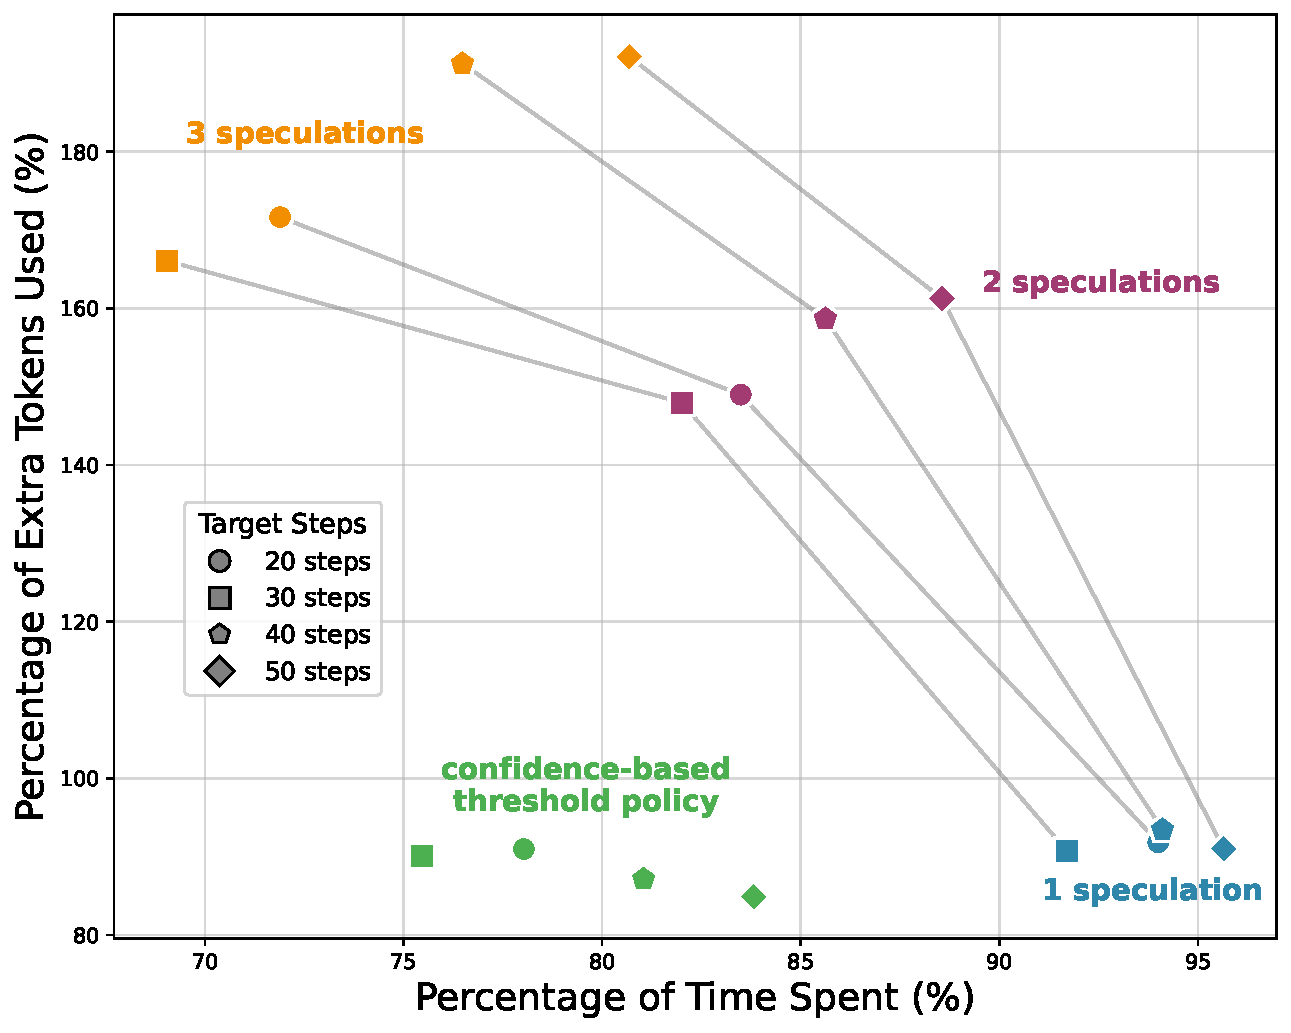
\includegraphics[width = 0.95\linewidth]{figures/chess/plot_with_confidence.pdf}
    \caption{Cost-latency tradeoff across different speculation widths, forming a Pareto curve.
    The confidence-based heuristic attains the lowest cost at latency comparable to three fixed predictions, outperforming fixed one- or two-branch strategies.
    }
    \vspace{-20pt}
    \label{fig:threshold}
\end{wrapfigure}
So far we assume a fixed branch accuracy $p$. In practice, we sometimes are able to obtain per-speculation confidence estimates (e.g., from intrinsic model logits, or from a separately-trained auxiliary predictor), allowing confidence-aware selective speculation. At each speculation window,
the accuracies of the $k$ speculative branches are random and drawn from a known distribution (which may vary over time). Before acting, the realized accuracy vector $\mathbf p = (p^1,\dots,p^k)$ is observed, and we choose how many of the top branches to launch.

We model the cost-latency tradeoff via the weighted objective
\begin{equation*}
    \max \; r\cdot\sum_{t=1}^T\mathrm{latency} - c\cdot\sum_{t=1}^T\mathrm{cost}
\end{equation*}
where $r$ and $c$ encode the relative importance of latency and cost. For simplicity, let $a$ and $b$ denote the fixed latency of the actor and speculator, and define the latency gain $\ell = r(a-b) > 0$.

% We again assume a fixed horizon $T$ and $k$-branch speculation. Suppose that at each time step, there is a known joint distribution $F_t$ from which the actual accuracy vector $\mathbf P_t = (P_t^1,\dots,P_t^k) \in [0,1]^k$ of each speculative branch is drawn from. Note that the distributions $F_t$ can vary across time step. At time step $t$, if currently there is a speculation window, i.e., the previous step did not result in a hit and thus this step is a cached action, then we observe an instantiated accuracy vector $\mathbf P_t = (P_t^1,\dots,P_t^k) \in [0,1]^k$. Based on these observed accuracies, our goal is to select a subset of these branches to accept. 

If the top $m$ branches are launched, the probability of a cached step is
$
q(m;\mathbf p)
=
1 - \prod_{j=1}^{m}(1-p^{(j)}),
$
where $p^{(1)} \ge \dots \ge p^{(k)}$ are the sorted confidences.

% \begin{theorem}[Finite-horizon two-mode dynamic program]
% \label{thm:dynamic-general}
% There exist scalars $\Delta_t$ (computed by backward recursion)
% such that at each speculation window $t$, after observing $\mathbf p$,
% the optimal number of branches satisfies
% \[
% m_t^\star(\mathbf p)
% \in
% \arg\max_{m \in \{0,\dots,k\}}
% \{ q(m;\mathbf p)\,\Delta_t - c m \},
% \]
% The continuation value $\Delta_t$ satisfies
% \[
% \Delta_T = 0, 
% \qquad
% \Delta_t
% =
% \ell
% -
% \mathbb E
% \Big[
% \max_m \{ q(m;\mathbf P)\,\Delta_{t+1} - c m \}
% \Big]\quad t=T-1, \dots, 1
% \]
% \end{theorem}
% The key implication is structural: \emph{dynamic selective speculation reduces to a one-dimensional trade-off}. 
% At each window, additional branches are launched only if their incremental hit probably, scaled by the continuation value $\Delta_t$, exceeds the per-branch cost $c$. All intertemporal effects are summarized by the single scalar $\Delta_t$.

% Furthermore, under stationary (the distribution of the accuracies is homogeneous) average-reward approximation, the structure simplifies further.

% \begin{corollary}[Stationary threshold rule (informal)]
% \label{cor:stationary-approximation}
% There exists a constant
% $\Delta^\star$ such that at any speculation window,
% the optimal breadth satisfies
% $m^\star(\mathbf p)
% \in
% \arg\max_{m}
% \{ q(m;\mathbf p)\,\Delta^\star - c m \}$. Equivalently, branches are added greedily in descending confidence order
% while $\Delta^\star \cdot \delta q(m;\mathbf p) \ge c$, with $\delta$ denoting the marginal gain from adding one more branch.
% \end{corollary}
% \paragraph{Practical takeaway.}
% The policy reduces to estimating a single scalar $\Delta^\star$ offline
% (e.g., from the stationary average-reward analysis).
% At runtime, given the confidences, the system sorts them
% and incrementally adds branches while the marginal gain in hit probability,
% scaled by $\Delta^\star$, exceeds the per-branch cost $c$.
% This requires only $O(k)$ computation per step and avoids solving a
% dynamic program online.
\vspace{10pt}
\begin{theorem}[Confidence-aware selective speculation]
\label{thm:dynamic-general}
There exist scalars $\Delta_t$ such that at each speculation window $t$, the optimal breadth satisfies
\[
m_t^\star(\mathbf p)
\in
\arg\max_{m \in \{0,\dots,k\}}
\{ q(m;\mathbf p)\,\Delta_t - c m \}.
\]
The continuation values are given by the backward recursion
\[
\Delta_T = 0, \qquad
\Delta_{1::T-1}
=
\ell
-
\mathbb E
\Big[
\max_m \{ q(m;\mathbf P)\,\Delta_{t+1} - c m \}
\Big]
\]
In the stationary case (time-homogeneous accuracy distribution), the continuation values 
$\Delta_t$ collapse to a single constant $\Delta^\star$. Thus branches are added greedily in descending confidence order
while
$\Delta^\star \cdot \delta q(m;\mathbf p) \ge c$, 
where $\delta q(m;\mathbf p)$ is the marginal gain from adding one more branch.
\label{thm:dynamic}
\end{theorem}
\paragraph{Interpretation and implementation}
The key implication is structural: dynamic selection collapses to a one-dimensional trade-off. 
Additional branches are launched only when their incremental hit probability,
scaled by a single continuation value ($\Delta_t$ or $\Delta^\star$),
exceeds the marginal cost $c$.
Under stationarity, this reduces to estimating $\Delta^\star$ offline;
at runtime, the system simply sorts confidences and adds branches greedily,
requiring $O(k)$ computation per step.

\paragraph{Empirical results} We implement a simple constant-threshold approximation of the stationary rule in the chess environment. At each step, after generating speculative branches, we use a predictor to estimate the correctness probability of each branch and continue only with those whose predicted accuracy exceeds 50\%. This implements a simplified threshold rule consistent with the structure suggested by Theorem~\ref{thm:dynamic}. Our method achieves the \emph{lowest additional token cost} while providing \emph{greater latency reduction} than naively launching 1 or 2 speculations per step.
\subsection{Depth-focused speculation} 
\label{subsec:depth-focused}
The previous two strategies are breadth-focused: each speculation is immediately followed by a real API call (speculative depth 1). Additionally, we analyze the opposite extreme: a \emph{depth-focused} policy, in which multi-step speculations are continuously spawned. Somewhat counterintuitively, this strategy does \emph{not} lead to exponential branch growth. Speculative calls are only extended when either a speculative or real call returns, and inconsistent subtrees are immediately pruned. Consequently, the system can run at most $a/b$ speculative steps ahead (governed by the relative speeds of real vs. speculative calls), ensuring that the number of active branches remains bounded and \emph{does not scale with the horizon $T$}. Under this policy, we can show that (formal theorem in Appendix~\ref{thm:depth})
\[
    \frac{\E[T_{\mathrm{seq}} - T_{\mathrm{spec}}]}{\E[T_{\mathrm{seq}}]}
    = \frac{T-1}{T} \, p \Bigl(1 - \frac{b}{a}\Bigr),\qquad
    \frac{\E[M_{\mathrm{spec}} - M_{\mathrm{seq}}]}{\E[M_{\mathrm{seq}}]}
    \approx\frac{T-1}{T}\left((1-p)\left(\frac{a}{2b}-\frac{1}{2}\right)+p\right)
\]
Compared to breadth speculation, depth speculation improves the latency coefficient from $\frac{p}{1+p}$ to $p$, increasing the theoretical speedup ceiling from $\frac{1}{2}$ to $1$. 
The cost term scales with $(1-p)(\frac{a}{2b}-\frac{1}{2})$, which captures how many speculative steps can accumulate before the real response arrives. 

% \subsection{Depth-focused speculation.} 
% \label{subsec:depth-focused}
% The previous two strategies are breadth-focused: each speculation is immediately followed by a real API call (speculative depth 1). Additionally, we analyze the opposite extreme: a \emph{depth-focused} policy, in which multi-step speculations are continuously spawned. Somewhat counterintuitively, this strategy does \emph{not} lead to a unbounded exponential blowup in the number of parallel branches. Speculative calls are only extended when either a speculative or real Actor call returns, and any subtree inconsistent with the real outcome is immediately pruned. Consequently, the system can run at most $a/b$ speculative steps ahead (governed by the relative speeds of real vs. speculative calls), ensuring that the number of active branches remains bounded and \emph{does not scale with the horizon $T$}.
% \begin{theorem}[Cost--Latency Tradeoff for Depth Speculation]
% Let $p$ be the baseline correctness probability of a speculative guess. Let $a$ and $b$ denote the fixed latency of real API and each speculation for simplicity. Using the same $T$ and $M$ notation, we have
% \[
%     \frac{\E[T_{\mathrm{seq}} - T_{\mathrm{spec}}]}{\E[T_{\mathrm{seq}}]}
%     = \frac{T-1}{T} \, p \Bigl(1 - \frac{b}{a}\Bigr),\qquad
%     \frac{\E[M_{\mathrm{spec}} - M_{\mathrm{seq}}]}{\E[M_{\mathrm{seq}}]}
%     \approx\frac{T-1}{T}\left((1-p)\left(\frac{a}{2b}+\frac{1}{2}\right)+p\frac{b}{a}\right)
% \]
% \end{theorem}


% This result highlights two contrasts with breadth speculation.
% First, the latency-speedup coefficient improves from $\frac{p}{1+p}$ (breadth) to $p$ (depth), raising the theoretical upper limit from $\tfrac{1}{2}$ to $1$. Second, the key term in the cost ratio, $(1-p)(\tfrac{a}{2b}+\tfrac{1}{2})$, reflects how many speculative steps can be launched before the real Actor response arrives. In the limit of perfect speculative accuracy, the ratio simplifies to $b/a$, corresponding to the extra cost of attaching a single speculative call to each real action.
